\lecture{16}{04.16}
\subsubsection*{独立组分数}%
\label{subsub:独立组分数}
\begin{defi}
    能够组成该化学环境的最少物质种类
\end{defi}
记独立组分数为$C$,物种数为$S$ ,存在化学平衡数为$R$
\begin{eg}
    对反应:\[
        \ce{NH_4HCO_3(s)}\ce{<=>[][]} \ce{NH_3(g)}+\ce{CO_2(g)}+\ce{H_2O(g)}
    .\]
    物种数$S=4$ ,有一个平衡$R=1$ ,三个同相物质相互约束$R'=2$ ,则独立组分数$C=S-R-R'=1$
\end{eg}
\subsubsection*{自由度}%
\label{subsub*:自由度}
系统的可变因素的数目(温度、压强、浓度等,不引起旧相消失和新相生成)
\begin{notation}
    条件自由度:指定某个强度变量,除该变量以外的其他自由度
\end{notation}
\begin{eg}
    指定$p$ ,条件自由度$f^\star $为$f^\star =f-1=2$
\end{eg}
\begin{eg}
    常温下液态数可以在一定范围内任意改变温度和压力而不改变相,因此自由度$f=2$
\end{eg}
\begin{notation}
    自由度随相数和独立组分数变化,由\textbf{相律}描述
\end{notation}
\subsubsection*{相律}%
\label{subsub*:相律}
\begin{equation}
    \label{eq:ffc2}
    f^\star + \Phi = C+2
\end{equation}
对于凝聚系统:压力影响不大,只有温度影响平衡:\begin{equation}
    \label{eq:fsfc1}
    f^\star +\Phi = C+1
\end{equation}
如果还要考虑其他因素:\begin{equation}
    \label{eq:ffcn}
    f + \Phi = C+n
\end{equation}
\begin{eg}
    计算一个系统的自由度:若NaCl(s)、NaCl溶液和水蒸气共存,求$f$ :

    由题$\Phi=3$ ,$C=2$ ,由相律$f = C+2-\Phi = 2$
\end{eg}
\subsection{相平衡条件}%
\label{sub:相平衡条件}
对于有$\Phi$ 个相的热力学平衡,包含共四个平衡:
\begin{itemize}
    \item 热平衡,使用温度衡量:$T_{\alpha}= T_{\beta}$
    \item 力学平衡,使用压强衡量:$p_{\alpha} = p_{\beta}$ 
    \item 相平衡,使用化学势衡量:$\mu_{\alpha}=\mu_{\beta}$
    \item 化学平衡,使用自由能衡量:$\Delta_\text{}G = 0 $
\end{itemize}
\subsection{Clausius-Clapeyron方程}%
\label{sub:Clausius-Clapeyron方程}
\[
    \frac{\mathrm{d}\ln p}{\mathrm{d}T} = \frac{\Delta_\text{vap}H_{m} }{RT} 
.\]
其中$\Delta_\text{vap}H_{m} $ 为摩尔气化焓,条件为气液两相平衡、气体为理想气体、液体体积忽略不计,积分后:
\begin{equation}
    \label{eq:int-clausius}
    \ln \frac{p_2}{p_1} = \frac{\Delta_\text{vap}H_{m} R}{\frac{1}{T_1}-\frac{1}{T_2}}
\end{equation}
使用该方程式从两个温度下的蒸汽压求摩尔气化焓
\subsection{水的相图}%
\label{sub:水的相图}
\begin{figure}[htpb]
    \centering
    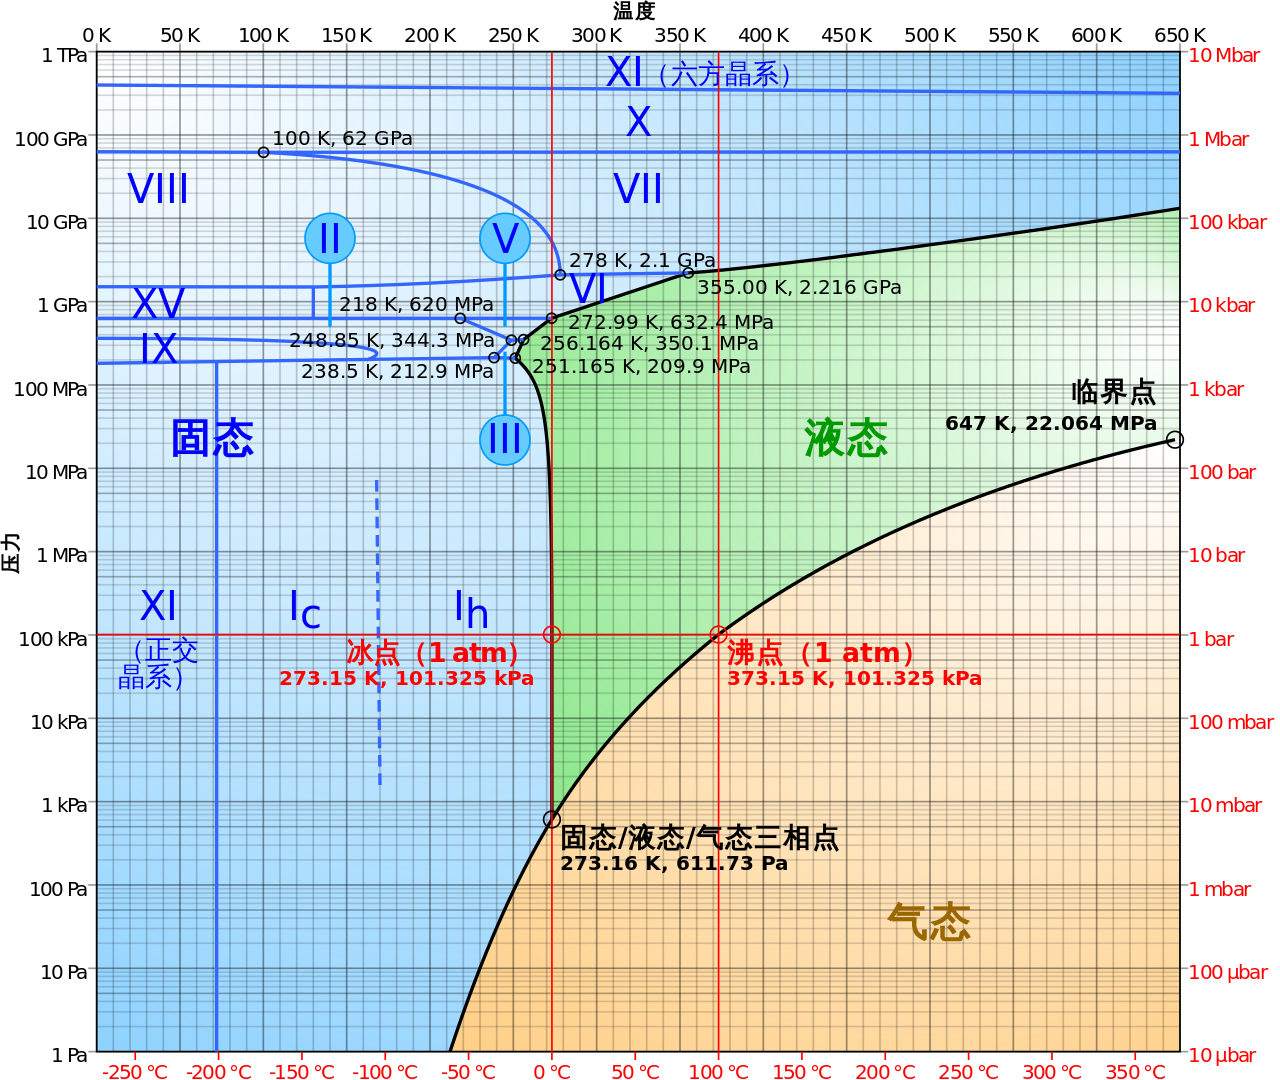
\includegraphics[width=0.8\textwidth]{./figures/水的相图.png}
    \caption{水的相图}
    \label{fig:figures-水的相图-png}
\end{figure}
在单相区域$\Phi=1,f=2$ 内,温度和压力独立有限度变化不会导致相的改变;在线上表示两相共存$\Phi=2,f=1$ ,压力和温度只能改变一个,其余由系统自行决定
